% id: 0175
% book: RPM 중3-2 수학 · 02 삼각비의 활용
% section: 유형 01 직각삼각형의 변의 길이 구하기
% figure: crop:fig-0175.png
% answer: ⑤
% answer_source: 답지
% variant_level: 0 (원본 전사)
% 이 파일은 build.mjs 가 items.json 에서 만든다. 고칠 때는 items.json 을 고친다.
\noindent\begin{minipage}[t]{0.58\linewidth}\vspace{0pt}\raggedright 오른쪽 그림의 직각삼각형~$\pt{ABC}$에서 다음 중 $x$, $y$의 값을 나타내는 것은?\end{minipage}\hfill\begin{minipage}[t]{0.4\linewidth}\vspace{0pt}\centering \setlength{\dmfigw}{76.1pt}\ifdim\dmfigw>\linewidth\setlength{\dmfigw}{\linewidth}\fi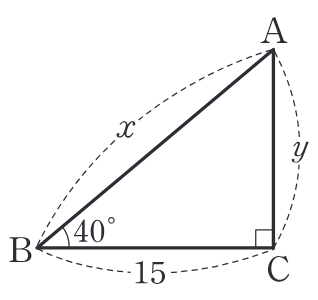
\includegraphics[width=\dmfigw]{figures/fig-0175.png}\end{minipage}\par
\begin{choicesv}{$x=15\sin 40^\circ$, $y=15\cos 40^\circ$}{$x=\dfrac{15}{\cos 40^\circ}$, $y=15\sin 40^\circ$}{$x=15\cos 40^\circ$, $y=15\tan 40^\circ$}{$x=15\cos 40^\circ$, $y=\dfrac{15}{\tan 40^\circ}$}{$x=\dfrac{15}{\cos 40^\circ}$, $y=15\tan 40^\circ$}\end{choicesv}
